\documentclass{standalone}
\usepackage{tikz}
\usetikzlibrary{patterns, positioning}


\begin{document}
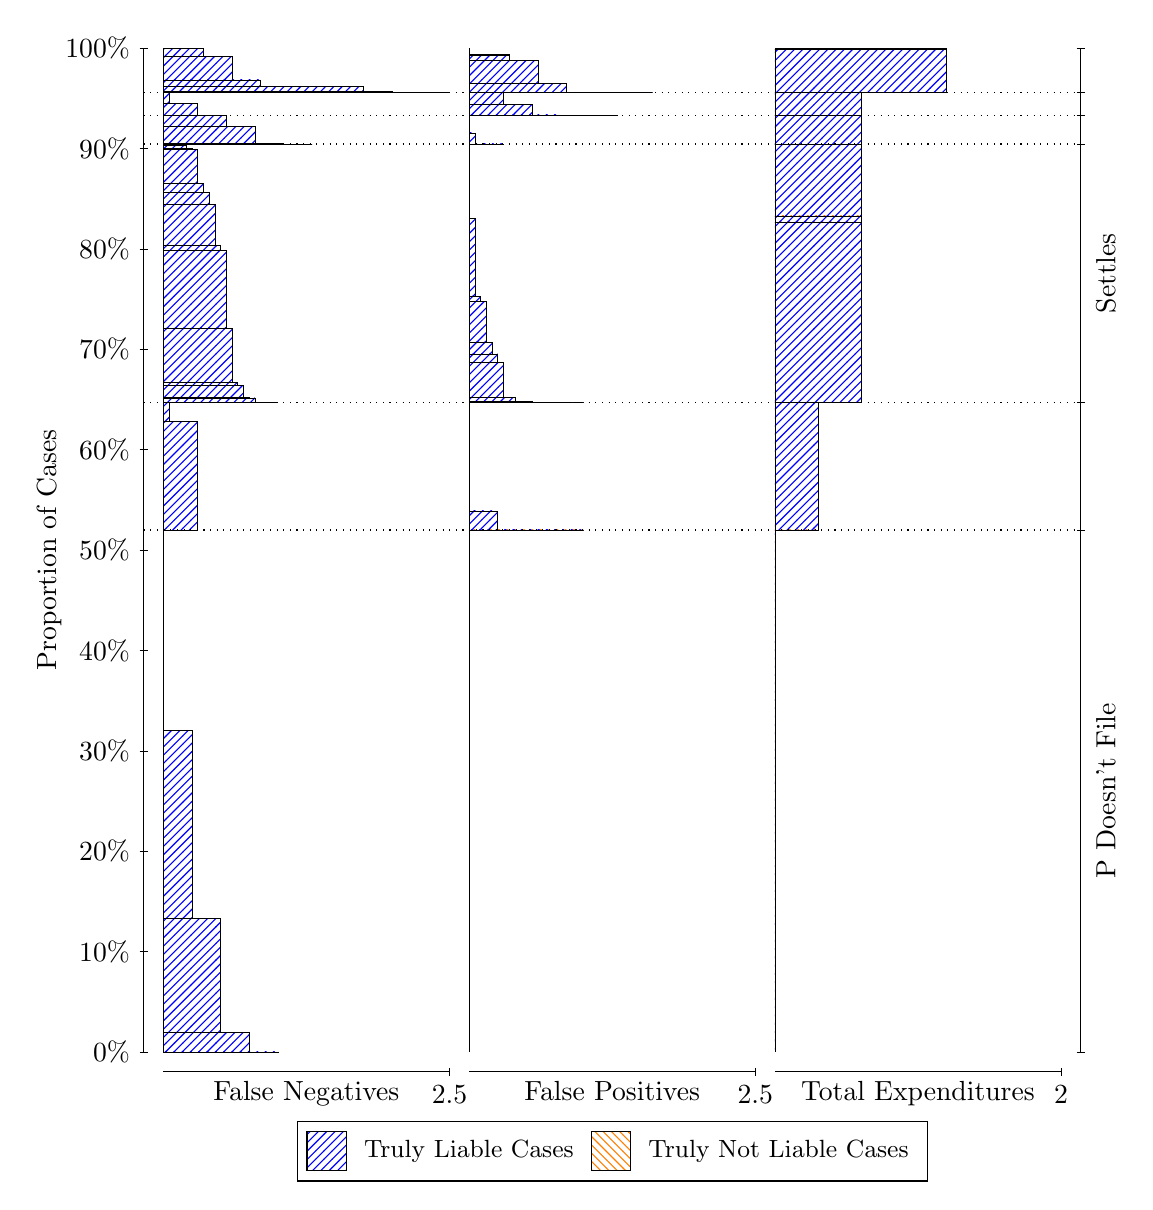
\begin{tikzpicture}
\draw[black, very thin] (1.5,1.75) -- (1.5,14.5);
\node[rotate=90, text=black, anchor=center] at (0.3, 8.125) {Proportion of Cases};
\draw[black, very thin] (1.45,1.75) -- (1.55,1.75);
\node[text=black, anchor=east] at (1.45, 1.75) {0\%};
\draw[black, very thin] (1.45,3.025) -- (1.55,3.025);
\node[text=black, anchor=east] at (1.45, 3.025) {10\%};
\draw[black, very thin] (1.45,4.3) -- (1.55,4.3);
\node[text=black, anchor=east] at (1.45, 4.3) {20\%};
\draw[black, very thin] (1.45,5.575) -- (1.55,5.575);
\node[text=black, anchor=east] at (1.45, 5.575) {30\%};
\draw[black, very thin] (1.45,6.85) -- (1.55,6.85);
\node[text=black, anchor=east] at (1.45, 6.85) {40\%};
\draw[black, very thin] (1.45,8.125) -- (1.55,8.125);
\node[text=black, anchor=east] at (1.45, 8.125) {50\%};
\draw[black, very thin] (1.45,9.4) -- (1.55,9.4);
\node[text=black, anchor=east] at (1.45, 9.4) {60\%};
\draw[black, very thin] (1.45,10.675) -- (1.55,10.675);
\node[text=black, anchor=east] at (1.45, 10.675) {70\%};
\draw[black, very thin] (1.45,11.95) -- (1.55,11.95);
\node[text=black, anchor=east] at (1.45, 11.95) {80\%};
\draw[black, very thin] (1.45,13.225) -- (1.55,13.225);
\node[text=black, anchor=east] at (1.45, 13.225) {90\%};
\draw[black, very thin] (1.45,14.5) -- (1.55,14.5);
\node[text=black, anchor=east] at (1.45, 14.5) {100\%};

\draw[black, very thin] (13.4,1.75) -- (13.4,14.5);
\draw[black, very thin] (13.35,1.75) -- (13.45,1.75);
\node[anchor=west] at (13.35, 1.75) {};
\draw[black, very thin] (13.35,8.3793) -- (13.45,8.3793);
\node[anchor=west] at (13.35, 8.3793) {};
\draw[black, very thin] (13.35,10) -- (13.45,10);
\node[anchor=west] at (13.35, 10) {};
\draw[black, very thin] (13.35,13.281) -- (13.45,13.281);
\node[anchor=west] at (13.35, 13.281) {};
\draw[black, very thin] (13.35,13.648) -- (13.45,13.648);
\node[anchor=west] at (13.35, 13.648) {};
\draw[black, very thin] (13.35,13.937) -- (13.45,13.937);
\node[anchor=west] at (13.35, 13.937) {};
\draw[black, very thin] (13.35,14.5) -- (13.45,14.5);
\node[anchor=west] at (13.35, 14.5) {};

\draw[black, very thin, pattern color=blue, pattern=north east lines] (1.75,1.75) rectangle (3.2033,1.7525);
\draw[black, very thin, pattern color=blue, pattern=north east lines] (1.75,1.7525) rectangle (2.84,1.9968);
\draw[black, very thin, pattern color=blue, pattern=north east lines] (1.75,1.9968) rectangle (2.4767,3.4452);
\draw[black, very thin, pattern color=blue, pattern=north east lines] (1.75,3.4452) rectangle (2.1133,5.8309);
\draw[black, very thin, pattern color=orange, pattern=north west lines] (1.75,5.8309) rectangle (1.75,5.8309);
\draw[black, very thin, pattern color=blue, pattern=north east lines] (1.75,5.8309) rectangle (1.75,8.3793);
\draw[black, very thin, pattern color=blue, pattern=north east lines] (1.75,8.3793) rectangle (2.186,9.7573);
\draw[black, very thin, pattern color=blue, pattern=north east lines] (1.75,9.7573) rectangle (1.8227,9.9995);
\draw[black, very thin, pattern color=orange, pattern=north west lines] (1.75,9.9995) rectangle (1.75,9.9995);
\draw[black, very thin, pattern color=blue, pattern=north east lines] (1.75,9.9995) rectangle (1.75,10);
\draw[black, very thin, pattern color=blue, pattern=north east lines] (1.75,10) rectangle (3.2033,10);
\draw[black, very thin, pattern color=blue, pattern=north east lines] (1.75,10) rectangle (3.058,10.001);
\draw[black, very thin, pattern color=blue, pattern=north east lines] (1.75,10.001) rectangle (2.9127,10.057);
\draw[black, very thin, pattern color=blue, pattern=north east lines] (1.75,10.057) rectangle (2.84,10.061);
\draw[black, very thin, pattern color=blue, pattern=north east lines] (1.75,10.061) rectangle (2.7673,10.22);
\draw[black, very thin, pattern color=blue, pattern=north east lines] (1.75,10.22) rectangle (2.6947,10.256);
\draw[black, very thin, pattern color=blue, pattern=north east lines] (1.75,10.256) rectangle (2.622,10.945);
\draw[black, very thin, pattern color=blue, pattern=north east lines] (1.75,10.945) rectangle (2.5493,11.929);
\draw[black, very thin, pattern color=blue, pattern=north east lines] (1.75,11.929) rectangle (2.4767,11.998);
\draw[black, very thin, pattern color=blue, pattern=north east lines] (1.75,11.998) rectangle (2.404,12.513);
\draw[black, very thin, pattern color=blue, pattern=north east lines] (1.75,12.513) rectangle (2.3313,12.665);
\draw[black, very thin, pattern color=blue, pattern=north east lines] (1.75,12.665) rectangle (2.2587,12.777);
\draw[black, very thin, pattern color=blue, pattern=north east lines] (1.75,12.777) rectangle (2.186,13.217);
\draw[black, very thin, pattern color=blue, pattern=north east lines] (1.75,13.217) rectangle (2.1133,13.221);
\draw[black, very thin, pattern color=blue, pattern=north east lines] (1.75,13.221) rectangle (2.0407,13.264);
\draw[black, very thin, pattern color=blue, pattern=north east lines] (1.75,13.264) rectangle (1.968,13.271);
\draw[black, very thin, pattern color=blue, pattern=north east lines] (1.75,13.271) rectangle (1.8953,13.271);
\draw[black, very thin, pattern color=blue, pattern=north east lines] (1.75,13.271) rectangle (1.8227,13.281);
\draw[black, very thin, pattern color=orange, pattern=north west lines] (1.75,13.281) rectangle (1.75,13.281);
\draw[black, very thin, pattern color=blue, pattern=north east lines] (1.75,13.281) rectangle (1.75,13.281);
\draw[black, very thin, pattern color=blue, pattern=north east lines] (1.75,13.281) rectangle (3.6393,13.281);
\draw[black, very thin, pattern color=blue, pattern=north east lines] (1.75,13.281) rectangle (3.276,13.287);
\draw[black, very thin, pattern color=blue, pattern=north east lines] (1.75,13.287) rectangle (2.9127,13.506);
\draw[black, very thin, pattern color=blue, pattern=north east lines] (1.75,13.506) rectangle (2.5493,13.647);
\draw[black, very thin, pattern color=blue, pattern=north east lines] (1.75,13.647) rectangle (2.186,13.648);
\draw[black, very thin, pattern color=orange, pattern=north west lines] (1.75,13.648) rectangle (1.75,13.648);
\draw[black, very thin, pattern color=blue, pattern=north east lines] (1.75,13.648) rectangle (2.186,13.801);
\draw[black, very thin, pattern color=blue, pattern=north east lines] (1.75,13.801) rectangle (1.8227,13.935);
\draw[black, very thin, pattern color=orange, pattern=north west lines] (1.75,13.935) rectangle (1.75,13.935);
\draw[black, very thin, pattern color=blue, pattern=north east lines] (1.75,13.935) rectangle (1.75,13.937);
\draw[black, very thin, pattern color=blue, pattern=north east lines] (1.75,13.937) rectangle (5.3833,13.937);
\draw[black, very thin, pattern color=blue, pattern=north east lines] (1.75,13.937) rectangle (5.02,13.937);
\draw[black, very thin, pattern color=blue, pattern=north east lines] (1.75,13.937) rectangle (4.6567,13.95);
\draw[black, very thin, pattern color=blue, pattern=north east lines] (1.75,13.95) rectangle (4.2933,14.009);
\draw[black, very thin, pattern color=blue, pattern=north east lines] (1.75,14.009) rectangle (3.93,14.014);
\draw[black, very thin, pattern color=blue, pattern=north east lines] (1.75,14.014) rectangle (3.712,14.014);
\draw[black, very thin, pattern color=blue, pattern=north east lines] (1.75,14.014) rectangle (3.5667,14.014);
\draw[black, very thin, pattern color=blue, pattern=north east lines] (1.75,14.014) rectangle (3.3487,14.014);
\draw[black, very thin, pattern color=blue, pattern=north east lines] (1.75,14.014) rectangle (3.2033,14.014);
\draw[black, very thin, pattern color=blue, pattern=north east lines] (1.75,14.014) rectangle (2.9853,14.095);
\draw[black, very thin, pattern color=blue, pattern=north east lines] (1.75,14.095) rectangle (2.622,14.391);
\draw[black, very thin, pattern color=blue, pattern=north east lines] (1.75,14.391) rectangle (2.2587,14.496);
\draw[black, very thin, pattern color=blue, pattern=north east lines] (1.75,14.496) rectangle (1.8953,14.5);
\draw[black, very thin, pattern color=orange, pattern=north west lines] (1.75,14.5) rectangle (1.75,14.5);
\draw[black, very thin, pattern color=blue, pattern=north east lines] (1.75,14.5) rectangle (1.75,14.5);
\draw[black, very thin, pattern color=orange, pattern=north west lines] (5.6333,1.75) rectangle (5.6333,1.75);
\draw[black, very thin, pattern color=blue, pattern=north east lines] (5.6333,1.75) rectangle (5.6333,8.3793);
\draw[black, very thin, pattern color=orange, pattern=north west lines] (5.6333,8.3793) rectangle (7.0867,8.3793);
\draw[black, very thin, pattern color=blue, pattern=north east lines] (5.6333,8.3793) rectangle (7.0867,8.3793);
\draw[black, very thin, pattern color=blue, pattern=north east lines] (5.6333,8.3793) rectangle (6.7233,8.3793);
\draw[black, very thin, pattern color=blue, pattern=north east lines] (5.6333,8.3793) rectangle (6.36,8.3803);
\draw[black, very thin, pattern color=blue, pattern=north east lines] (5.6333,8.3803) rectangle (5.9967,8.6224);
\draw[black, very thin, pattern color=blue, pattern=north east lines] (5.6333,8.6224) rectangle (5.6333,10);
\draw[black, very thin, pattern color=orange, pattern=north west lines] (5.6333,10) rectangle (7.0867,10);
\draw[black, very thin, pattern color=blue, pattern=north east lines] (5.6333,10) rectangle (7.0867,10);
\draw[black, very thin, pattern color=orange, pattern=north west lines] (5.6333,10) rectangle (6.9413,10);
\draw[black, very thin, pattern color=blue, pattern=north east lines] (5.6333,10) rectangle (6.9413,10);
\draw[black, very thin, pattern color=orange, pattern=north west lines] (5.6333,10) rectangle (6.796,10);
\draw[black, very thin, pattern color=blue, pattern=north east lines] (5.6333,10) rectangle (6.796,10);
\draw[black, very thin, pattern color=blue, pattern=north east lines] (5.6333,10) rectangle (6.7233,10);
\draw[black, very thin, pattern color=orange, pattern=north west lines] (5.6333,10) rectangle (6.6507,10);
\draw[black, very thin, pattern color=blue, pattern=north east lines] (5.6333,10) rectangle (6.6507,10);
\draw[black, very thin, pattern color=blue, pattern=north east lines] (5.6333,10) rectangle (6.578,10.001);
\draw[black, very thin, pattern color=orange, pattern=north west lines] (5.6333,10.001) rectangle (6.5053,10.001);
\draw[black, very thin, pattern color=blue, pattern=north east lines] (5.6333,10.001) rectangle (6.5053,10.001);
\draw[black, very thin, pattern color=blue, pattern=north east lines] (5.6333,10.001) rectangle (6.4327,10.01);
\draw[black, very thin, pattern color=blue, pattern=north east lines] (5.6333,10.01) rectangle (6.36,10.011);
\draw[black, very thin, pattern color=blue, pattern=north east lines] (5.6333,10.011) rectangle (6.2873,10.017);
\draw[black, very thin, pattern color=blue, pattern=north east lines] (5.6333,10.017) rectangle (6.2147,10.06);
\draw[black, very thin, pattern color=blue, pattern=north east lines] (5.6333,10.06) rectangle (6.142,10.064);
\draw[black, very thin, pattern color=blue, pattern=north east lines] (5.6333,10.064) rectangle (6.0693,10.504);
\draw[black, very thin, pattern color=blue, pattern=north east lines] (5.6333,10.504) rectangle (5.9967,10.616);
\draw[black, very thin, pattern color=blue, pattern=north east lines] (5.6333,10.616) rectangle (5.924,10.768);
\draw[black, very thin, pattern color=blue, pattern=north east lines] (5.6333,10.768) rectangle (5.8513,11.283);
\draw[black, very thin, pattern color=blue, pattern=north east lines] (5.6333,11.283) rectangle (5.7787,11.352);
\draw[black, very thin, pattern color=blue, pattern=north east lines] (5.6333,11.352) rectangle (5.706,12.336);
\draw[black, very thin, pattern color=blue, pattern=north east lines] (5.6333,12.336) rectangle (5.6333,13.281);
\draw[black, very thin, pattern color=orange, pattern=north west lines] (5.6333,13.281) rectangle (6.0693,13.281);
\draw[black, very thin, pattern color=blue, pattern=north east lines] (5.6333,13.281) rectangle (6.0693,13.282);
\draw[black, very thin, pattern color=blue, pattern=north east lines] (5.6333,13.282) rectangle (5.706,13.423);
\draw[black, very thin, pattern color=blue, pattern=north east lines] (5.6333,13.423) rectangle (5.6333,13.648);
\draw[black, very thin, pattern color=orange, pattern=north west lines] (5.6333,13.648) rectangle (7.5227,13.648);
\draw[black, very thin, pattern color=blue, pattern=north east lines] (5.6333,13.648) rectangle (7.5227,13.648);
\draw[black, very thin, pattern color=blue, pattern=north east lines] (5.6333,13.648) rectangle (7.1593,13.648);
\draw[black, very thin, pattern color=blue, pattern=north east lines] (5.6333,13.648) rectangle (6.796,13.65);
\draw[black, very thin, pattern color=blue, pattern=north east lines] (5.6333,13.65) rectangle (6.4327,13.784);
\draw[black, very thin, pattern color=blue, pattern=north east lines] (5.6333,13.784) rectangle (6.0693,13.937);
\draw[black, very thin, pattern color=orange, pattern=north west lines] (5.6333,13.937) rectangle (7.9587,13.937);
\draw[black, very thin, pattern color=blue, pattern=north east lines] (5.6333,13.937) rectangle (7.9587,13.937);
\draw[black, very thin, pattern color=orange, pattern=north west lines] (5.6333,13.937) rectangle (7.5953,13.937);
\draw[black, very thin, pattern color=blue, pattern=north east lines] (5.6333,13.937) rectangle (7.5953,13.937);
\draw[black, very thin, pattern color=orange, pattern=north west lines] (5.6333,13.937) rectangle (7.232,13.937);
\draw[black, very thin, pattern color=blue, pattern=north east lines] (5.6333,13.937) rectangle (7.232,13.941);
\draw[black, very thin, pattern color=blue, pattern=north east lines] (5.6333,13.941) rectangle (6.8687,14.046);
\draw[black, very thin, pattern color=orange, pattern=north west lines] (5.6333,14.046) rectangle (6.8687,14.046);
\draw[black, very thin, pattern color=blue, pattern=north east lines] (5.6333,14.046) rectangle (6.8687,14.046);
\draw[black, very thin, pattern color=blue, pattern=north east lines] (5.6333,14.046) rectangle (6.5053,14.34);
\draw[black, very thin, pattern color=blue, pattern=north east lines] (5.6333,14.34) rectangle (6.5053,14.342);
\draw[black, very thin, pattern color=blue, pattern=north east lines] (5.6333,14.342) rectangle (6.142,14.407);
\draw[black, very thin, pattern color=blue, pattern=north east lines] (5.6333,14.407) rectangle (6.142,14.423);
\draw[black, very thin, pattern color=orange, pattern=north west lines] (5.6333,14.423) rectangle (5.924,14.423);
\draw[black, very thin, pattern color=blue, pattern=north east lines] (5.6333,14.423) rectangle (5.924,14.423);
\draw[black, very thin, pattern color=blue, pattern=north east lines] (5.6333,14.423) rectangle (5.7787,14.423);
\draw[black, very thin, pattern color=blue, pattern=north east lines] (5.6333,14.423) rectangle (5.7787,14.423);
\draw[black, very thin, pattern color=orange, pattern=north west lines] (5.6333,14.423) rectangle (5.6333,14.423);
\draw[black, very thin, pattern color=blue, pattern=north east lines] (5.6333,14.423) rectangle (5.6333,14.5);
\draw[black, very thin, pattern color=orange, pattern=north west lines] (9.5167,1.75) rectangle (9.5167,1.75);
\draw[black, very thin, pattern color=blue, pattern=north east lines] (9.5167,1.75) rectangle (9.5167,8.3793);
\draw[black, very thin, pattern color=orange, pattern=north west lines] (9.5167,8.3793) rectangle (10.062,8.3793);
\draw[black, very thin, pattern color=blue, pattern=north east lines] (9.5167,8.3793) rectangle (10.062,10);
\draw[black, very thin, pattern color=orange, pattern=north west lines] (9.5167,10) rectangle (10.607,10);
\draw[black, very thin, pattern color=blue, pattern=north east lines] (9.5167,10) rectangle (10.607,12.293);
\draw[black, very thin, pattern color=orange, pattern=north west lines] (9.5167,12.293) rectangle (10.607,12.293);
\draw[black, very thin, pattern color=blue, pattern=north east lines] (9.5167,12.293) rectangle (10.607,12.369);
\draw[black, very thin, pattern color=orange, pattern=north west lines] (9.5167,12.369) rectangle (10.607,12.369);
\draw[black, very thin, pattern color=blue, pattern=north east lines] (9.5167,12.369) rectangle (10.607,13.281);
\draw[black, very thin, pattern color=orange, pattern=north west lines] (9.5167,13.281) rectangle (10.607,13.281);
\draw[black, very thin, pattern color=blue, pattern=north east lines] (9.5167,13.281) rectangle (10.607,13.648);
\draw[black, very thin, pattern color=orange, pattern=north west lines] (9.5167,13.648) rectangle (10.607,13.648);
\draw[black, very thin, pattern color=blue, pattern=north east lines] (9.5167,13.648) rectangle (10.607,13.937);
\draw[black, very thin, pattern color=orange, pattern=north west lines] (9.5167,13.937) rectangle (11.697,13.937);
\draw[black, very thin, pattern color=blue, pattern=north east lines] (9.5167,13.937) rectangle (11.697,14.482);
\draw[black, very thin, pattern color=orange, pattern=north west lines] (9.5167,14.482) rectangle (11.697,14.482);
\draw[black, very thin, pattern color=blue, pattern=north east lines] (9.5167,14.482) rectangle (11.697,14.5);
\draw[black, dotted] (1.5,8.3793) -- (13.4,8.3793);
\draw[black, dotted] (1.5,10) -- (13.4,10);
\draw[black, dotted] (1.5,13.281) -- (13.4,13.281);
\draw[black, dotted] (1.5,13.648) -- (13.4,13.648);
\draw[black, dotted] (1.5,13.937) -- (13.4,13.937);
\draw[black, very thin] (1.75,1.5) -- (5.3833,1.5);
\node[text=black, anchor=north] at (3.5667, 1.5) {False Negatives};
\draw[black, very thin] (5.3833,1.45) -- (5.3833,1.55);
\node[text=black, anchor=north] at (5.3833, 1.45) {2.5};

\draw[black, very thin] (5.6333,1.5) -- (9.2667,1.5);
\node[text=black, anchor=north] at (7.45, 1.5) {False Positives};
\draw[black, very thin] (9.2667,1.45) -- (9.2667,1.55);
\node[text=black, anchor=north] at (9.2667, 1.45) {2.5};

\draw[black, very thin] (9.5167,1.5) -- (13.15,1.5);
\node[text=black, anchor=north] at (11.333, 1.5) {Total Expenditures};
\draw[black, very thin] (13.15,1.45) -- (13.15,1.55);
\node[text=black, anchor=north] at (13.15, 1.45) {2};

\node[text=black, centered, rotate=90] at (13.72, 5.0646) {P Doesn't File};

\node[text=black, centered, rotate=90] at (13.72, 11.641) {Settles};




\draw (7.449999999999999,1.5) node[draw=none] (baseCoordinate) {};
\begin{scope}[align=center]
        \matrix[scale=0.5, draw=black, below=0.5cm of baseCoordinate, nodes={draw}, column sep=0.1cm]{
            \node[rectangle, draw, minimum width=0.5cm, minimum height=0.5cm, pattern color=blue, pattern=north east lines] {}; &
            \node[draw=none, font=\small, text=black] (B) {Truly Liable Cases}; &
            \node[rectangle, draw, minimum width=0.5cm, minimum height=0.5cm, pattern color=orange, pattern=north west lines] {}; &
            \node[draw=none, font=\small, text=black] (B) {Truly Not Liable Cases}; \\
            };
\end{scope}

\end{tikzpicture}
\end{document}